\documentclass{article}
\usepackage{graphicx}
\usepackage{amsmath}
\usepackage{amssymb}
\usepackage{hyperref}
\usepackage{biblatex}
\usepackage[a4paper]{geometry}
\usepackage{float}
\usepackage[export]{adjustbox}
\usepackage{wrapfig}

\bibliography{Image Processing Project}

\author{Netanel Madmoni}

\title{Intro to Image Processing Course Final Project \\
\large Investigating the Effects of Image Enhancement Techniques 
on the Performance of rPPG Models for
Physiological Signals Extraction from Facial Videos}

\begin{document}

\maketitle

\section*{Introduction}

\begin{wrapfigure}{r}{0.5\textwidth}
	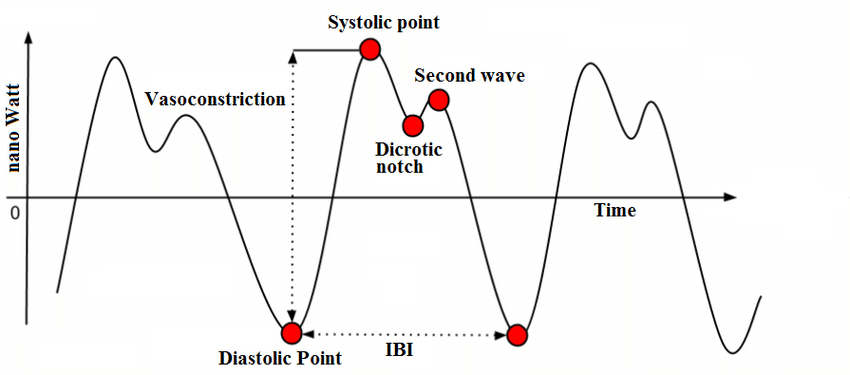
\includegraphics[scale=0.25]{figures/A-typical-PPG-signal-and-its-components.png}
	\caption{A typical PPG signal and its components. Source: \cite{nathPhotoplethysmogramBasedNonInvasive2018}}
\end{wrapfigure}

Photoplethysmography (PPG) is a common method for displaying blood volume changes over time. First described in the 1930s, PPG signals are widely used nowadays as they provide helpful insights on one's cardiac, respiratory and autonomic systems. Traditionally PPG signal are obtained by placing a device called a \textit{photoelectric plethysmograph} right over the subject's hand (typically on one of the fingers). The device consists of a light source and a light detector; It shines a light through the skin and then measures the light absorption of it over time \cite{alianPhotoplethysmography2014}. The signal is cyclic, since each heart beat makes the blood vessels under the skin to expand and contract, which affects the amount of light absorbed. Therefore, signal allows measurement of vital signs such as heart rate, heart rate variability, and oxygen saturation \cite{pirzadaRemotePhotoplethysmographyRPPG2023}.

Remote Photoplethysmography (rPPG) is a camera-drived method of obtaining an PPG signal in a remote fashion. It relies on the subtle changes in the color of the subject's face over time to extract a signal, which is later cleaned and processed \cite{pirzadaRemotePhotoplethysmographyRPPG2023}. In the last decades a variety of models were developed for extracting a quality signal and processing it to get reliable results. In recent years with the increased popularity of deep learning methods, more and more researches attempt to utilize the power of neural networks for this task.



\section*{Project Overview}

In this project we aim to investigate the effects of several image processing techniques on the performance of rPPG models.

Given a video clip of a person’s face $\mathbf{X}$ and parameters $\mathbf{\Theta}$, create an image enhancer model $f_{1}(\mathbf{X} | \mathbf{\Theta})$ to enhance the video frames, and use a signal extractor model $f_{2}(f_{1}(\mathbf{X} | \mathbf{\Theta}))$ that will extract the PPG signal $\hat{y}$ from it, so that the error between extracted signal $\hat{y}$ and true signal $y$ is minimal.

For a flowchart describing the project's main pipeline, see Figure \ref{fig:flowchart}.

\begin{figure}[H]
	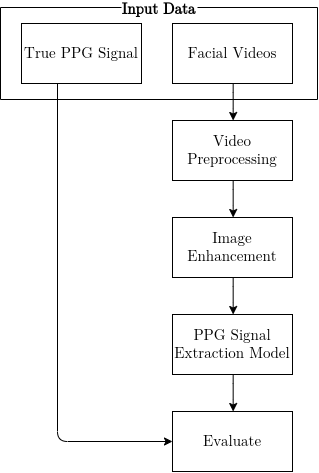
\includegraphics[scale=0.45, center]{figures/flowchart.png}
	\caption{A flowchart describing the main data processing pipeline.}
	\label{fig:flowchart}
\end{figure}

\subsection*{Image Enhancement Techniques to be Explored}

\begin{itemize}
	\item Color space conversion
	\item Thresholding
	\item Image sharpening, unsharp mask
	\item Wavelet processing
	\item Histogram transformations
	\item Histogram stretching, Histogram equalization, CLAHE, Log transform, Contrast stretching, Thresholding, Histogram matching, Linear noise smoothing with a kernel
	\item Edge detection
	\item Morphological operations (Erosion, Dilation, Opening, Closing, Morphological gradient, Black hat, Top hat)
	\item Image pyramids (Gaussian and Laplacian), Image Blending using Pyramids
	\item Image filtering (various filters)
	\item Image Segmentation
\end{itemize}

\section*{Data}
For the data we will use a publicly available rPPG dataset, such as the
\href{https://data.4tu.nl/articles/dataset/Public_Benchmark_Dataset_for_Testing_rPPG_Algorithm_Performance/12684059/1}{Public Benchmark Dataset for Testing rPPG Algorithm Performance}, the \href{https://sites.google.com/view/ybenezeth/ubfcrppg}{UBFCrPPG Dataset}, or a different data source (to be decided).

\section*{Limitations}

Our biggest limitation in this project is computing power and training time. We will take the necessary steps to better suit the data to fit our available resources and time, such as downsampling the data or using a subset of it.

\printbibliography

\end{document}